% Options for packages loaded elsewhere
\PassOptionsToPackage{unicode}{hyperref}
\PassOptionsToPackage{hyphens}{url}
%
\documentclass[
  ignorenonframetext,
]{beamer}
\usepackage{pgfpages}
\setbeamertemplate{caption}[numbered]
\setbeamertemplate{caption label separator}{: }
\setbeamercolor{caption name}{fg=normal text.fg}
\beamertemplatenavigationsymbolsempty
% Prevent slide breaks in the middle of a paragraph
\widowpenalties 1 10000
\raggedbottom
\setbeamertemplate{part page}{
  \centering
  \begin{beamercolorbox}[sep=16pt,center]{part title}
    \usebeamerfont{part title}\insertpart\par
  \end{beamercolorbox}
}
\setbeamertemplate{section page}{
  \centering
  \begin{beamercolorbox}[sep=12pt,center]{part title}
    \usebeamerfont{section title}\insertsection\par
  \end{beamercolorbox}
}
\setbeamertemplate{subsection page}{
  \centering
  \begin{beamercolorbox}[sep=8pt,center]{part title}
    \usebeamerfont{subsection title}\insertsubsection\par
  \end{beamercolorbox}
}
\AtBeginPart{
  \frame{\partpage}
}
\AtBeginSection{
  \ifbibliography
  \else
    \frame{\sectionpage}
  \fi
}
\AtBeginSubsection{
  \frame{\subsectionpage}
}

\usepackage{amsmath,amssymb}
\usepackage{lmodern}
\usepackage{iftex}
\ifPDFTeX
  \usepackage[T1]{fontenc}
  \usepackage[utf8]{inputenc}
  \usepackage{textcomp} % provide euro and other symbols
\else % if luatex or xetex
  \usepackage{unicode-math}
  \defaultfontfeatures{Scale=MatchLowercase}
  \defaultfontfeatures[\rmfamily]{Ligatures=TeX,Scale=1}
  \setmonofont[]{JuliaMono}
\fi
% Use upquote if available, for straight quotes in verbatim environments
\IfFileExists{upquote.sty}{\usepackage{upquote}}{}
\IfFileExists{microtype.sty}{% use microtype if available
  \usepackage[]{microtype}
  \UseMicrotypeSet[protrusion]{basicmath} % disable protrusion for tt fonts
}{}
\makeatletter
\@ifundefined{KOMAClassName}{% if non-KOMA class
  \IfFileExists{parskip.sty}{%
    \usepackage{parskip}
  }{% else
    \setlength{\parindent}{0pt}
    \setlength{\parskip}{6pt plus 2pt minus 1pt}}
}{% if KOMA class
  \KOMAoptions{parskip=half}}
\makeatother
\usepackage{xcolor}
\newif\ifbibliography
\setlength{\emergencystretch}{3em} % prevent overfull lines
\setcounter{secnumdepth}{-\maxdimen} % remove section numbering

\usepackage{color}
\usepackage{fancyvrb}
\newcommand{\VerbBar}{|}
\newcommand{\VERB}{\Verb[commandchars=\\\{\}]}
\DefineVerbatimEnvironment{Highlighting}{Verbatim}{commandchars=\\\{\}}
% Add ',fontsize=\small' for more characters per line
\usepackage{framed}
\definecolor{shadecolor}{RGB}{241,243,245}
\newenvironment{Shaded}{\begin{snugshade}}{\end{snugshade}}
\newcommand{\AlertTok}[1]{\textcolor[rgb]{0.68,0.00,0.00}{#1}}
\newcommand{\AnnotationTok}[1]{\textcolor[rgb]{0.37,0.37,0.37}{#1}}
\newcommand{\AttributeTok}[1]{\textcolor[rgb]{0.40,0.45,0.13}{#1}}
\newcommand{\BaseNTok}[1]{\textcolor[rgb]{0.68,0.00,0.00}{#1}}
\newcommand{\BuiltInTok}[1]{\textcolor[rgb]{0.00,0.23,0.31}{#1}}
\newcommand{\CharTok}[1]{\textcolor[rgb]{0.13,0.47,0.30}{#1}}
\newcommand{\CommentTok}[1]{\textcolor[rgb]{0.37,0.37,0.37}{#1}}
\newcommand{\CommentVarTok}[1]{\textcolor[rgb]{0.37,0.37,0.37}{\textit{#1}}}
\newcommand{\ConstantTok}[1]{\textcolor[rgb]{0.56,0.35,0.01}{#1}}
\newcommand{\ControlFlowTok}[1]{\textcolor[rgb]{0.00,0.23,0.31}{#1}}
\newcommand{\DataTypeTok}[1]{\textcolor[rgb]{0.68,0.00,0.00}{#1}}
\newcommand{\DecValTok}[1]{\textcolor[rgb]{0.68,0.00,0.00}{#1}}
\newcommand{\DocumentationTok}[1]{\textcolor[rgb]{0.37,0.37,0.37}{\textit{#1}}}
\newcommand{\ErrorTok}[1]{\textcolor[rgb]{0.68,0.00,0.00}{#1}}
\newcommand{\ExtensionTok}[1]{\textcolor[rgb]{0.00,0.23,0.31}{#1}}
\newcommand{\FloatTok}[1]{\textcolor[rgb]{0.68,0.00,0.00}{#1}}
\newcommand{\FunctionTok}[1]{\textcolor[rgb]{0.28,0.35,0.67}{#1}}
\newcommand{\ImportTok}[1]{\textcolor[rgb]{0.00,0.46,0.62}{#1}}
\newcommand{\InformationTok}[1]{\textcolor[rgb]{0.37,0.37,0.37}{#1}}
\newcommand{\KeywordTok}[1]{\textcolor[rgb]{0.00,0.23,0.31}{#1}}
\newcommand{\NormalTok}[1]{\textcolor[rgb]{0.00,0.23,0.31}{#1}}
\newcommand{\OperatorTok}[1]{\textcolor[rgb]{0.37,0.37,0.37}{#1}}
\newcommand{\OtherTok}[1]{\textcolor[rgb]{0.00,0.23,0.31}{#1}}
\newcommand{\PreprocessorTok}[1]{\textcolor[rgb]{0.68,0.00,0.00}{#1}}
\newcommand{\RegionMarkerTok}[1]{\textcolor[rgb]{0.00,0.23,0.31}{#1}}
\newcommand{\SpecialCharTok}[1]{\textcolor[rgb]{0.37,0.37,0.37}{#1}}
\newcommand{\SpecialStringTok}[1]{\textcolor[rgb]{0.13,0.47,0.30}{#1}}
\newcommand{\StringTok}[1]{\textcolor[rgb]{0.13,0.47,0.30}{#1}}
\newcommand{\VariableTok}[1]{\textcolor[rgb]{0.07,0.07,0.07}{#1}}
\newcommand{\VerbatimStringTok}[1]{\textcolor[rgb]{0.13,0.47,0.30}{#1}}
\newcommand{\WarningTok}[1]{\textcolor[rgb]{0.37,0.37,0.37}{\textit{#1}}}

\providecommand{\tightlist}{%
  \setlength{\itemsep}{0pt}\setlength{\parskip}{0pt}}\usepackage{longtable,booktabs,array}
\usepackage{calc} % for calculating minipage widths
\usepackage{caption}
% Make caption package work with longtable
\makeatletter
\def\fnum@table{\tablename~\thetable}
\makeatother
\usepackage{graphicx}
\makeatletter
\def\maxwidth{\ifdim\Gin@nat@width>\linewidth\linewidth\else\Gin@nat@width\fi}
\def\maxheight{\ifdim\Gin@nat@height>\textheight\textheight\else\Gin@nat@height\fi}
\makeatother
% Scale images if necessary, so that they will not overflow the page
% margins by default, and it is still possible to overwrite the defaults
% using explicit options in \includegraphics[width, height, ...]{}
\setkeys{Gin}{width=\maxwidth,height=\maxheight,keepaspectratio}
% Set default figure placement to htbp
\makeatletter
\def\fps@figure{htbp}
\makeatother

\makeatletter
\makeatother
\makeatletter
\makeatother
\makeatletter
\@ifpackageloaded{caption}{}{\usepackage{caption}}
\AtBeginDocument{%
\ifdefined\contentsname
  \renewcommand*\contentsname{Table of contents}
\else
  \newcommand\contentsname{Table of contents}
\fi
\ifdefined\listfigurename
  \renewcommand*\listfigurename{List of Figures}
\else
  \newcommand\listfigurename{List of Figures}
\fi
\ifdefined\listtablename
  \renewcommand*\listtablename{List of Tables}
\else
  \newcommand\listtablename{List of Tables}
\fi
\ifdefined\figurename
  \renewcommand*\figurename{Figure}
\else
  \newcommand\figurename{Figure}
\fi
\ifdefined\tablename
  \renewcommand*\tablename{Table}
\else
  \newcommand\tablename{Table}
\fi
}
\@ifpackageloaded{float}{}{\usepackage{float}}
\floatstyle{ruled}
\@ifundefined{c@chapter}{\newfloat{codelisting}{h}{lop}}{\newfloat{codelisting}{h}{lop}[chapter]}
\floatname{codelisting}{Listing}
\newcommand*\listoflistings{\listof{codelisting}{List of Listings}}
\makeatother
\makeatletter
\@ifpackageloaded{caption}{}{\usepackage{caption}}
\@ifpackageloaded{subcaption}{}{\usepackage{subcaption}}
\makeatother
\makeatletter
\@ifpackageloaded{tcolorbox}{}{\usepackage[many]{tcolorbox}}
\makeatother
\makeatletter
\@ifundefined{shadecolor}{\definecolor{shadecolor}{rgb}{.97, .97, .97}}
\makeatother
\makeatletter
\makeatother
\ifLuaTeX
  \usepackage{selnolig}  % disable illegal ligatures
\fi
\IfFileExists{bookmark.sty}{\usepackage{bookmark}}{\usepackage{hyperref}}
\IfFileExists{xurl.sty}{\usepackage{xurl}}{} % add URL line breaks if available
\urlstyle{same} % disable monospaced font for URLs
\hypersetup{
  pdftitle={Brain Modelling},
  pdfauthor={Nicholas Gale \& Stephen Eglen},
  hidelinks,
  pdfcreator={LaTeX via pandoc}}

\title{Brain Modelling}
\subtitle{How brains process information.}
\author{Nicholas Gale \& Stephen Eglen}
\date{}

\begin{document}
\frame{\titlepage}
\ifdefined\Shaded\renewenvironment{Shaded}{\begin{tcolorbox}[enhanced, boxrule=0pt, interior hidden, frame hidden, borderline west={3pt}{0pt}{shadecolor}, sharp corners, breakable]}{\end{tcolorbox}}\fi

\begin{frame}{Brain Modelling.}
\protect\hypertarget{brain-modelling.}{}
\begin{itemize}
\item
  Deep Learning is most often applied as a statistical model to
  understand data.
\item
  Deep Learning is a branch of \emph{theoretical neuroscience} which
  aims to model brain function and development.
\item
  It is therefore useful to understand some modelling results from
  theoretical neuroscience.
\item
  We will start by covering some basic brain biology.
\end{itemize}
\end{frame}

\begin{frame}{The Brain}
\protect\hypertarget{the-brain}{}
\begin{itemize}
\item
  A common view is that the brain is a statistical model.
\item
  Takes input as sensory data and output as thoughts/muscle
  movements/etc.
\item
  A good base to develop models on but the brain is \emph{incredibly}
  complex and models are \emph{simple}.
\item
  At a basic level it consists of \(\approx 10^9\) specialised cells
  called \emph{neurons}.
\item
  These neurons signal with each other to perform computations.
\item
  Computations are often localised in brain regions called modules
  e.g.~visual cortex.
\end{itemize}
\end{frame}

\begin{frame}{Neurons}
\protect\hypertarget{neurons}{}
\begin{columns}[T]
\begin{column}{0.5\textwidth}
\begin{itemize}
\item
  Neurons thought of in terms of: soma, axon, dendrite.
\item
  Soma is the cell body.
\item
  Axon is a long protrusion connecting to other cells.
\item
  Dendrites connect to axons of other cells and integrate signals.
\end{itemize}
\end{column}

\begin{column}{0.5\textwidth}
\begin{figure}

{\centering \includegraphics{./images/neuron_anatomy.png}

}

\caption{Neuron Anatomy}

\end{figure}
\end{column}
\end{columns}
\end{frame}

\begin{frame}{Membrane Voltage}
\protect\hypertarget{membrane-voltage}{}
\begin{itemize}
\item
  Neurons regulate themselves through a membrane voltage.
\item
  This is typically measued in mV and a common baseline is -55mV.
\item
  The voltage is controlled by gated ionic channels: Na, K, etc.
\item
  The membrane voltage can be regulated by current input.
\end{itemize}
\end{frame}

\begin{frame}{Spiking}
\protect\hypertarget{spiking}{}
\begin{columns}[T]
\begin{column}{0.5\textwidth}
\begin{itemize}
\item
  Spiking, or an \emph{action potential}, occurs at a threshold membrane
  voltage. Referred to as ``firing''.
\item
  It is a runaway reaction of rapid voltage increase: depolarisation.
\item
  Followed by a voltage decrease: hyper polarisation.
\item
  After an action potential there is a refractory period where the
  neuron cant fire.
\end{itemize}
\end{column}

\begin{column}{0.5\textwidth}
\includegraphics{./images/action_potential.jpg}
\end{column}
\end{columns}
\end{frame}

\begin{frame}{Signals}
\protect\hypertarget{signals}{}
\begin{itemize}
\item
  An action potential carries this change in voltage down the axon to
  other cells.
\item
  A neuron can fire many action potentials a second.
\item
  The combined pattern is a signal to other cells e.g.~``contract
  muscle''/``release''.
\end{itemize}
\end{frame}

\begin{frame}{Firing Patterns}
\protect\hypertarget{firing-patterns}{}
\begin{figure}

{\centering \includegraphics{./images/spiking_patterns.png}

}

\caption{\href{https://www.izhikevich.org/publications/spikes.html}{Common
Firing Patterns}}

\end{figure}
\end{frame}

\begin{frame}{Synapse}
\protect\hypertarget{synapse}{}
\begin{itemize}
\item
  The axon is connected to a dendrite through a synapse.
\item
  When an action potential reaches the synapse it releases charged
  neurotransmitters into the synaptic cleft.
\item
  These diffuse through the cleft to bind to the dendrite.
\item
  They modulate the dendrites voltage upward (excitatory) or downward
  (inhibitory).
\end{itemize}
\end{frame}

\begin{frame}{Networks}
\protect\hypertarget{networks}{}
\begin{itemize}
\item
  A neural network is simply the composition of many connected neurons.
\item
  The brain is a large neural network.
\item
  Subdivisions are also networks e.g.~auditory cortex, hippocampus etc.
\item
  The inputs to the network and synaptic weights modulate firing
  patterns of neurons.
\item
  The combined effect is to perform a computation on the inputs.
\end{itemize}
\end{frame}

\begin{frame}{Networks inspiration}
\protect\hypertarget{networks-inspiration}{}
\begin{itemize}
\item
  Reduced models of specific brain networks have been highly successful.
  \emph{Some} examples:
\item
  Visual system processing: Deep Convolutional Networks.
\item
  Generalised Feed-Forward Networks: Artificial Neural Network (the
  blueprint).
\item
  Cortical recurrent networks: Hopfield Networks (asscociative memory).
\item
  Visual system development: Optimisation Heuristics (Elastic Net).
\item
  Many more.
\end{itemize}
\end{frame}

\begin{frame}{Neuron Modelling}
\protect\hypertarget{neuron-modelling}{}
\begin{itemize}
\item
  The neurone is a highly complicated structure - even our best models
  are still reductions.
\item
  The oldest neuron models date to 1901.
\item
  They are almost all based on the law of conductance:
  \[ C\frac{dV}{dt} = I \]
\item
  Commonly classed as: integrate-and-fire, biophysical, hybrid, or
  stochastic.
\end{itemize}
\end{frame}

\begin{frame}{Integrate and Fire}
\protect\hypertarget{integrate-and-fire}{}
\begin{itemize}
\item
  The oldest form of neuron model.
\item
  Assume neuron conductance is \(g\): \[\frac{dv}{dt} = g I(t)\]
\item
  If \(I(t) = \sum_{t_i\in\text{spike times}} \delta(t - t_i)\) then
  this ``integrates'' the spikes into membrane voltage.
\item
  Once a threshold is reached, \(v\) is reset to a baseline.
\end{itemize}
\end{frame}

\begin{frame}[fragile]{Numerical Implementation:}
\protect\hypertarget{numerical-implementation}{}
\begin{columns}[T]
\begin{column}{0.5\textwidth}
\begin{Shaded}
\begin{Highlighting}[]
\ImportTok{using} \BuiltInTok{Plots}
\NormalTok{dt }\OperatorTok{=} \FloatTok{0.01}\NormalTok{; T }\OperatorTok{=} \FunctionTok{collect}\NormalTok{(}\FloatTok{0}\OperatorTok{:}\NormalTok{dt}\OperatorTok{:}\FloatTok{1}\NormalTok{);}
\NormalTok{iT }\OperatorTok{=} \FloatTok{0.25} \OperatorTok{.\textless{}}\NormalTok{ T }\OperatorTok{.\textless{}} \FloatTok{0.75}\NormalTok{;}
\NormalTok{ g }\OperatorTok{=} \FloatTok{1}\NormalTok{; thresh }\OperatorTok{=} \FloatTok{0.2}\NormalTok{; reset }\OperatorTok{=} \OperatorTok{{-}}\FloatTok{0.1}
\NormalTok{v }\OperatorTok{=} \FunctionTok{similar}\NormalTok{(T)}
\ControlFlowTok{for}\NormalTok{ t }\KeywordTok{in} \FloatTok{2}\OperatorTok{:}\FunctionTok{length}\NormalTok{(T)}
\NormalTok{    dv }\OperatorTok{=}\NormalTok{ g }\OperatorTok{*}\NormalTok{ iT[t]}
\NormalTok{    v[t] }\OperatorTok{=}\NormalTok{ v[t}\OperatorTok{{-}}\FloatTok{1}\NormalTok{] }\OperatorTok{+}\NormalTok{ dt }\OperatorTok{*}\NormalTok{ dv}
    \ControlFlowTok{if}\NormalTok{ v[t] }\OperatorTok{\textgreater{}}\NormalTok{ thresh}
\NormalTok{        v[t] }\OperatorTok{=}\NormalTok{ reset}
    \ControlFlowTok{end}
\ControlFlowTok{end}
\end{Highlighting}
\end{Shaded}
\end{column}

\begin{column}{0.5\textwidth}
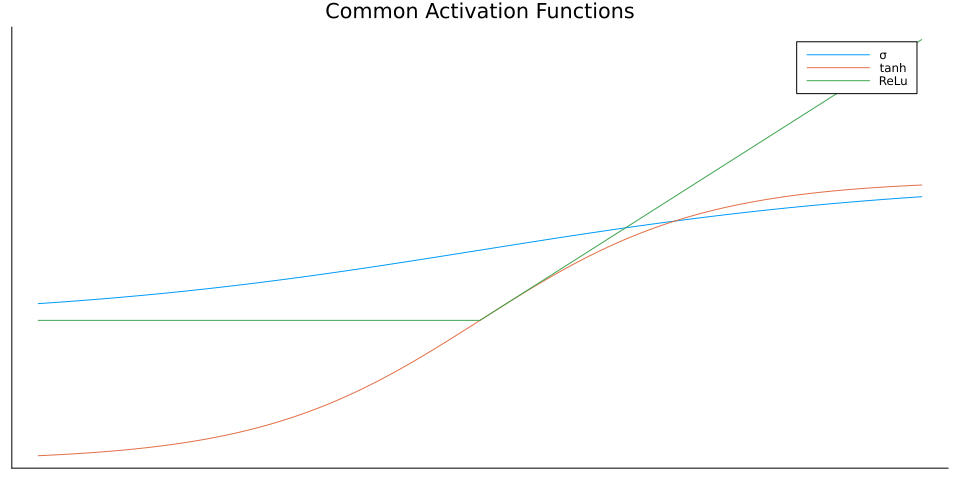
\includegraphics{lecture2_files/figure-beamer/cell-3-output-1.pdf}
\end{column}
\end{columns}
\end{frame}

\begin{frame}{Leaky Integrate and Fire}
\protect\hypertarget{leaky-integrate-and-fire}{}
\begin{itemize}
\item
  A slightly more sophisticated model recognises that a neuron tends to
  ``rest'' at a baseline.
\item
  If it doesn't fire its membrane voltage decays through ion channels
  diffusion.
\item
  To model this we assume a resting voltage of \(v_r\) and a
  differential equation: \[\frac{dv}{dt} = -g(v-v_r) + gI(t)\]
\end{itemize}
\end{frame}

\begin{frame}[fragile]{Numerical Implementation:}
\protect\hypertarget{numerical-implementation-1}{}
\begin{columns}[T]
\begin{column}{0.5\textwidth}
\begin{Shaded}
\begin{Highlighting}[]
\NormalTok{dt }\OperatorTok{=} \FloatTok{0.01}\NormalTok{; T }\OperatorTok{=} \FunctionTok{collect}\NormalTok{(}\FloatTok{0}\OperatorTok{:}\NormalTok{dt}\OperatorTok{:}\FloatTok{1}\NormalTok{);}
\NormalTok{iT }\OperatorTok{=} \FloatTok{0.1} \OperatorTok{.\textless{}}\NormalTok{ T }\OperatorTok{.\textless{}} \FloatTok{0.5}\NormalTok{; }
\NormalTok{g }\OperatorTok{=} \FloatTok{1}\NormalTok{; thresh }\OperatorTok{=} \FloatTok{0.05}\NormalTok{; reset }\OperatorTok{=} \OperatorTok{{-}}\FloatTok{0.2}
\NormalTok{vr }\OperatorTok{=} \OperatorTok{{-}}\FloatTok{0.05}\NormalTok{;}
\NormalTok{v }\OperatorTok{=} \FunctionTok{zeros}\NormalTok{(}\FunctionTok{length}\NormalTok{(T)) }\OperatorTok{.{-}} \FloatTok{0.1}
\ControlFlowTok{for}\NormalTok{ t }\KeywordTok{in} \FloatTok{2}\OperatorTok{:}\FunctionTok{length}\NormalTok{(T)}
\NormalTok{    dv }\OperatorTok{=}\NormalTok{ g }\OperatorTok{*}\NormalTok{ iT[t] }\OperatorTok{{-}}\NormalTok{ (v[t}\OperatorTok{{-}}\FloatTok{1}\NormalTok{]}\OperatorTok{{-}}\NormalTok{vr)}
\NormalTok{    v[t] }\OperatorTok{=}\NormalTok{ v[t}\OperatorTok{{-}}\FloatTok{1}\NormalTok{] }\OperatorTok{+}\NormalTok{ dt }\OperatorTok{*}\NormalTok{ dv}
    \ControlFlowTok{if}\NormalTok{ v[t] }\OperatorTok{\textgreater{}}\NormalTok{ thresh}
\NormalTok{        v[t] }\OperatorTok{=}\NormalTok{ reset}
    \ControlFlowTok{end}
\ControlFlowTok{end}
\end{Highlighting}
\end{Shaded}
\end{column}

\begin{column}{0.5\textwidth}
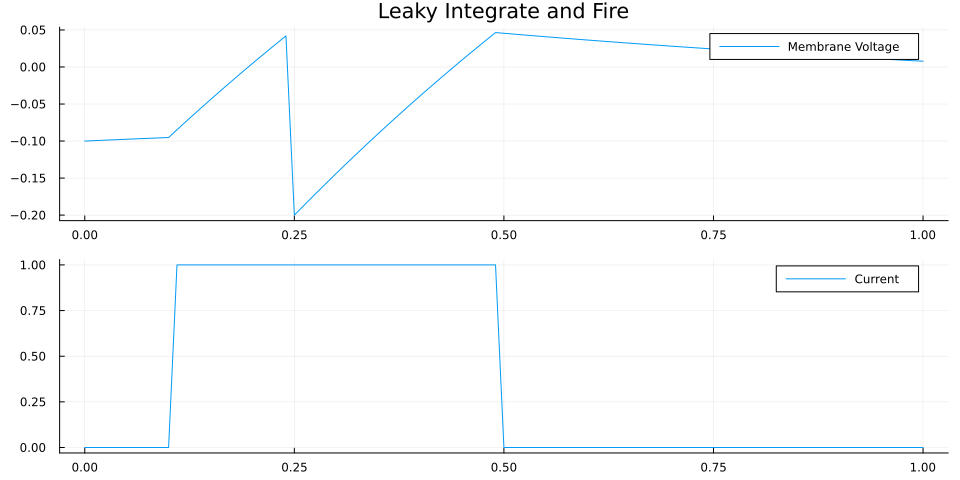
\includegraphics{lecture2_files/figure-beamer/cell-5-output-1.pdf}
\end{column}
\end{columns}
\end{frame}

\begin{frame}{Hodgkin-Huxley}
\protect\hypertarget{hodgkin-huxley}{}
\begin{itemize}
\item
  The Hodgkin-Huxley is a jewel of theoretical neuroscience (and
  modelling more generally).
\item
  It explicitly models Na and K ionic channels with condutances
  \(g_{Na}\) and \(g_{k}\) and a leaky channel \(g_L\).
\item
  It models the response of these channels to a membrane voltage through
  response variables: \(n,m,h\).
\item
  It does not require a ``hard-reset'' and is able to accurately predict
  neuron behaviour quantitatively.
\end{itemize}
\end{frame}

\begin{frame}{Hodgkin-Huxley Definition}
\protect\hypertarget{hodgkin-huxley-definition}{}
\begin{itemize}
\tightlist
\item
  The differential equations are as follows:
  \[ C \frac{dv}{dt} = g_K n_1^4 (v_K - v) + g_{Na} n_2^3 n_3 (v_{Na} - v) + g_L(v_L - v) + I(t) \]
  \[ \frac{dn}{dt} = \alpha_{n_i}(v)(1-n_i)+\beta_{n_i}(v)n_i \]
\end{itemize}
\end{frame}

\begin{frame}{}
\protect\hypertarget{section}{}
\begin{itemize}
\item
  The functions \(\alpha_j, \beta_j\) take the generic form:
  \[\frac{A_j (v - B_j)}{\exp\left(\frac{v-B_p}{C_p}\right) - D_p}\]
\item
  The parameters can be found by fitting to neural voltage data.
\end{itemize}

\begin{figure}

{\centering \includegraphics[width=\textwidth,height=0.4\textheight]{./images/hhneuronetrace.png}

}

\caption{\href{https://www.ncbi.nlm.nih.gov/pmc/articles/PMC3424716/}{Membrane
voltage of giant squid axon (top) against the model prediction
(bottom)}}

\end{figure}
\end{frame}

\begin{frame}{Hybrid Models}
\protect\hypertarget{hybrid-models}{}
\begin{itemize}
\item
  The Hodgkin-Huxley model is \emph{accurate} and has been extended for
  even more accuracy, but is \emph{expensive}.
\item
  The integrate-and-fire models are \emph{cheap}.
\item
  Hybrid models reduce the biophysical HH type models to blend
  efficiency and accuracy.
\item
  They usually consist of a voltage (v) and auxillary (u) variable. They
  can be useful in analtyical and computational frameworks.
\item
  The best in class is the Izhekivich model.
\end{itemize}
\end{frame}

\begin{frame}{Hybrid Model Fit}
\protect\hypertarget{hybrid-model-fit}{}
\begin{figure}

{\centering \includegraphics[width=\textwidth,height=0.6\textheight]{./images/izspike.png}

}

\caption{\href{https://www.izhikevich.org/publications/spikes.html}{Izhekivich
model spiking predictions compared to rat cortical neurons}}

\end{figure}
\end{frame}

\begin{frame}{Firing Rates}
\protect\hypertarget{firing-rates}{}
\begin{itemize}
\item
  All of the models presented can generate various classes of behaviour:
  quiet, single-spikes, periodic spikes.
\item
  Under constant current conditions periodic spiking can be described by
  the firing rate (Hz)
\item
  This is an important biological measurement and computational
  reduction.
\item
  A school of thought believes that the rate encodes the neurons
  computation: rate based computation.
\item
  There is evidence for this but it is simplistic. It does however form
  the basis of Deep Learning models.
\end{itemize}
\end{frame}

\begin{frame}{Stochastic}
\protect\hypertarget{stochastic}{}
\begin{itemize}
\item
  The final class of model is a stochastic model.
\item
  It asserts that neuron spiking is distributed as a Poisson process
  parameterised by firing rate \(r\): \[X \sim \text{Poisson}(r)\]
\end{itemize}
\end{frame}

\begin{frame}{Implementation}
\protect\hypertarget{implementation}{}
\begin{itemize}
\item
  A spike train is created by choosing a rate \(r\) and a time interval
  \(dt\).
\item
  At the \(N\)th time step (time \(t_0 + N dt\)) sample a uniform random
  number \(p\).
\item
  If \(p < r dt\) then record a spike.
\item
  This is the cheapest spiking model to implement.
\end{itemize}
\end{frame}

\begin{frame}{Inhomogeneous Poisson}
\protect\hypertarget{inhomogeneous-poisson}{}
\begin{itemize}
\item
  The inhomogenous process process allows \(r = r(t)\) if the rate
  changes slowly. \[X\sim\text{Poisson}(r(t)\]
\item
  This process captures most statistical properties of real neurons.
\item
  Stochastic process are a cheap way to generate spike data.
\end{itemize}
\end{frame}

\begin{frame}{Activation Functions}
\protect\hypertarget{activation-functions}{}
\begin{itemize}
\item
  A probabilistic intepretation leads us to relate rates/probabilities
  with membrane voltage
\item
  An activation function measures the ``activity'' of a neuron as a
  response to membrane voltage.
\item
  The most biologically accurate function is the sigmoid.
\end{itemize}
\end{frame}

\begin{frame}{Sigmoid Activation}
\protect\hypertarget{sigmoid-activation}{}
\begin{itemize}
\item
  Let the maximum firing rate of a neurone be Q; its threshold be
  \(\theta\); and slope-response to voltage be \(\beta\)
\item
  The sigmoid function \(s\) is given by:
  \[ s(x; \beta, Q, \theta) = \frac{Q}{1 + \exp\left(-\frac{x-\theta}{\beta}\right)}\]
\end{itemize}
\end{frame}

\begin{frame}{}
\protect\hypertarget{section-1}{}
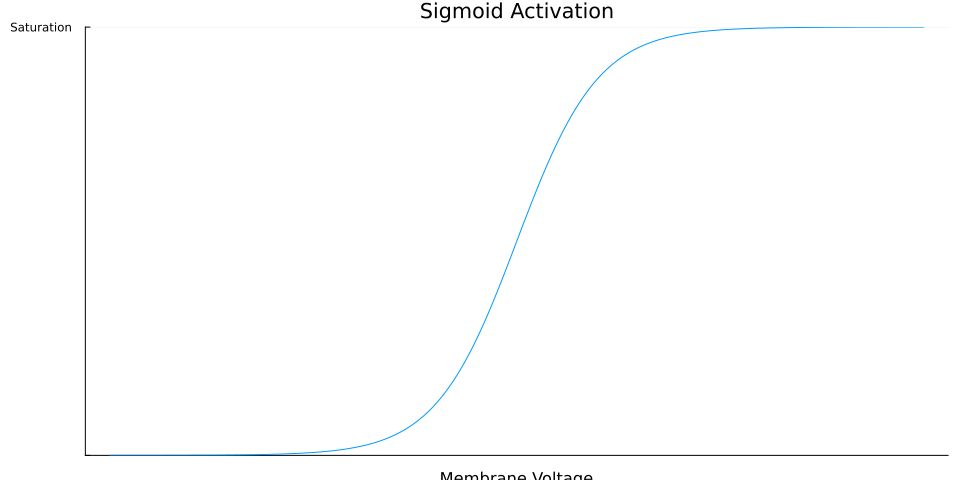
\includegraphics{lecture2_files/figure-beamer/cell-6-output-1.pdf}
\end{frame}

\begin{frame}{Common Activation Functions}
\protect\hypertarget{common-activation-functions}{}
\begin{itemize}
\item
  Other activation functions are commonly chosen.
\item
  These are less accurate but have nice mathematical/computational
  properties.
\item
  Tanh(x): a scaled sigmoid to be odd around the origin.
\item
  ramp(x): a computationally cheap approximation. Also called Rectified
  Linear Unit (relu)
\item
  Heaviside(x): a simple on/off intepretation that is useful in proofs.
\end{itemize}
\end{frame}

\begin{frame}{Tanh}
\protect\hypertarget{tanh}{}
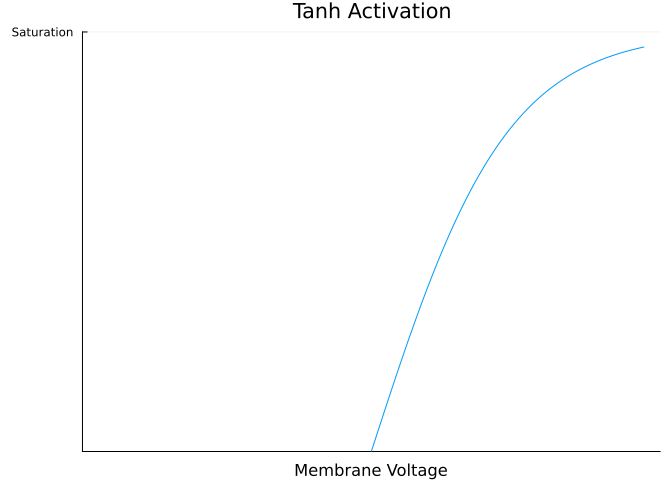
\includegraphics{lecture2_files/figure-beamer/cell-7-output-1.pdf}
\end{frame}

\begin{frame}{Ramp/Rectified Linear Unit (ReLu)}
\protect\hypertarget{ramprectified-linear-unit-relu}{}
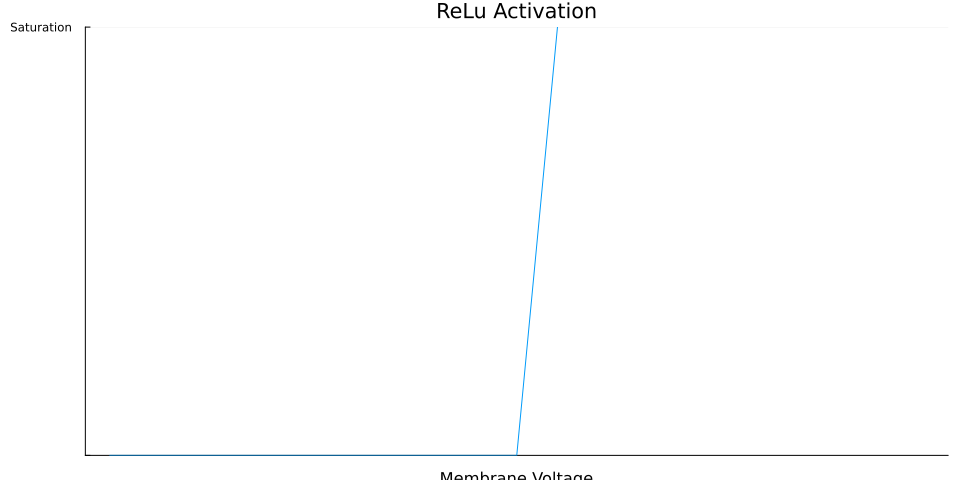
\includegraphics{lecture2_files/figure-beamer/cell-8-output-1.pdf}
\end{frame}

\begin{frame}{Heaviside}
\protect\hypertarget{heaviside}{}
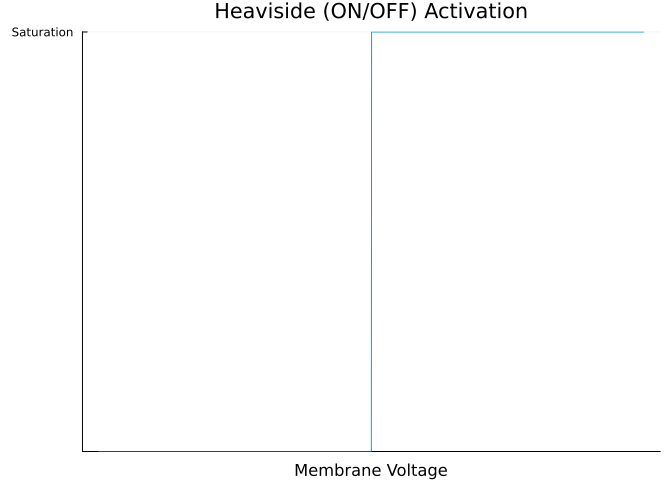
\includegraphics{lecture2_files/figure-beamer/cell-9-output-1.pdf}
\end{frame}

\begin{frame}{Neural Network Models}
\protect\hypertarget{neural-network-models}{}
\begin{itemize}
\item
  We have built up a sophisticated repotoire of neuron activity models.
\item
  We would like to build them into something more useful.
\item
  To do this we incoporate them into a dynamical network model.
\end{itemize}
\end{frame}

\begin{frame}{Networks}
\protect\hypertarget{networks-1}{}
\begin{itemize}
\item
  A network is simply a graph with nodes \(i \in 1:N\) and edges
  \(W_{ij}\).
\item
  A dynamical network model is composed of internal dynamics of the node
  and contributions from the edges.
\item
  It typically takes the form:
  \[\frac{dv_i}{dt} = f(v_i, t) + \sum_{j=1}{N} W_{ij} g(v_j, t) \]
\end{itemize}
\end{frame}

\begin{frame}{Dendrites}
\protect\hypertarget{dendrites}{}
\begin{itemize}
\item
  A neural network model replaces \(f\) with the activation dynamics and
  \(W_{ij}\) with the contributions from other neurons.
\item
  \(W_{ij}\) have a physical intepretation: they are dendritic weights.
\item
  g represents some response function such as spiking.
\item
  This is the most general form of a neural network.
\item
  \emph{All} of the above neurone models will be able to learn an input
  response.
\item
  The most common form is a linear response to weights passed through an
  some activation function.
\end{itemize}
\end{frame}

\begin{frame}{The Hopfield Network}
\protect\hypertarget{the-hopfield-network}{}
\begin{itemize}
\item
  The Hopfield Network is a seminal work in neural network theory.
\item
  It is a good statistical classifier.
\item
  It has a naturally intepretable structure.
\item
  It has a biologically derived learning rule and provides explanations
  for biological phenemona.
\item
  It therefore ticks \emph{all} the boxes.
\end{itemize}
\end{frame}

\begin{frame}{The Hopfield Network Setup:}
\protect\hypertarget{the-hopfield-network-setup}{}
\begin{itemize}
\item
  In the Hopfield model a pool of N cortical neurons are all connected
  to each other.
\item
  The neurons are indexed by \(i\) and the weights by \(W_{ij}\). The
  inputs are given to neurons as \(u_i^0 = I_i\).
\item
  The neurons state is evolved as
  \[u_i^{t+1} = \text{sign}(\sum_j W{ij} u_j^t)\]
\end{itemize}
\end{frame}

\begin{frame}{}
\protect\hypertarget{section-2}{}
\begin{itemize}
\item
  The sign function classifies neurons as active/inactive and the state
  is evolved until it is steady.
\item
  The steady state can be compared to a hashing function to classify an
  input.
\end{itemize}
\end{frame}

\begin{frame}{The Hebb rule: Training}
\protect\hypertarget{the-hebb-rule-training}{}
\begin{itemize}
\item
  The Hopfield network uses the Hebb rule to train its weights.
\item
  The Hebb rules states: neurons that fire together wire together. This
  means coactive neurons strengthen; otherwise they decay.
\item
  To encode an input pattern \(v\) we take the autocovariance as the
  weight change i.e.~the Hebb rule: \[ \Delta W_{ij} = v_i v_j \]
\end{itemize}
\end{frame}

\begin{frame}{}
\protect\hypertarget{section-3}{}
\begin{itemize}
\item
  The autocovariance relationship ensures that the steady state of the
  pattern v is v itself.
\item
  To train M such patterns we simply take the mean of the linear
  combinations of the Hebb rule.
\item
  We also hash the patterns for classification later.
\end{itemize}
\end{frame}

\begin{frame}[fragile]{Hopfield Network Training}
\protect\hypertarget{hopfield-network-training}{}
\begin{Shaded}
\begin{Highlighting}[numbers=left,,]
\ImportTok{using} \BuiltInTok{Random}
\FunctionTok{delW}\NormalTok{(v) }\OperatorTok{=} \FunctionTok{sign}\NormalTok{.(v) }\OperatorTok{.*} \FunctionTok{sign}\NormalTok{.(v)}\CharTok{\textquotesingle{}}
\KeywordTok{function} \FunctionTok{constructW}\NormalTok{(data)}
\NormalTok{    W }\OperatorTok{=} \FunctionTok{zeros}\NormalTok{(}\FunctionTok{length}\NormalTok{(data[}\FloatTok{1}\NormalTok{]), }\FunctionTok{length}\NormalTok{(data[}\FloatTok{1}\NormalTok{]))}
    \ControlFlowTok{for}\NormalTok{ v }\KeywordTok{in}\NormalTok{ data}
\NormalTok{        W }\OperatorTok{.+=} \FunctionTok{delW}\NormalTok{(v)}
    \ControlFlowTok{end}
    \ControlFlowTok{return}\NormalTok{ W }\OperatorTok{./} \FunctionTok{length}\NormalTok{(data)}
\KeywordTok{end}
\NormalTok{data }\OperatorTok{=}\NormalTok{ [}\FunctionTok{sign}\NormalTok{.(}\FunctionTok{rand}\NormalTok{([}\OperatorTok{{-}}\FloatTok{0.2}\NormalTok{, }\FloatTok{0.8}\NormalTok{], }\FloatTok{784}\NormalTok{)) for i }\KeywordTok{in} \FloatTok{1}\OperatorTok{:}\FloatTok{10}\NormalTok{]}
\NormalTok{labels }\OperatorTok{=}\NormalTok{ [}\FunctionTok{randstring}\NormalTok{(}\FloatTok{10}\NormalTok{) for i }\KeywordTok{in} \FloatTok{1}\OperatorTok{:}\FloatTok{10}\NormalTok{]}
\NormalTok{hash }\OperatorTok{=} \FunctionTok{Dict}\NormalTok{(}\FunctionTok{zip}\NormalTok{(data, labels))}
\NormalTok{trained }\OperatorTok{=} \FunctionTok{constructW}\NormalTok{(data)}
\end{Highlighting}
\end{Shaded}
\end{frame}

\begin{frame}{Partial Input}
\protect\hypertarget{partial-input}{}
\begin{itemize}
\item
  The Hopfield network can then be used to query inputs and classify
  them.
\item
  We find we can delete substantial portions of vectors and still
  classify them correctly.
\item
  We can also classify vectors that are ``similar''.
\end{itemize}
\end{frame}

\begin{frame}[fragile]{Partial Input: Prediction}
\protect\hypertarget{partial-input-prediction}{}
\begin{verbatim}
class_predict (generic function with 1 method)
\end{verbatim}

\begin{Shaded}
\begin{Highlighting}[]
\FunctionTok{corrupt}\NormalTok{(c) }\OperatorTok{=} \FunctionTok{map}\NormalTok{(x }\OperatorTok{{-}\textgreater{}}\NormalTok{ (}\FunctionTok{rand}\NormalTok{()}\OperatorTok{\textgreater{}}\FloatTok{0.5}\NormalTok{) ? x }\OperatorTok{:} \FunctionTok{{-}sign}\NormalTok{(x) }\OperatorTok{*} \FunctionTok{rand}\NormalTok{(), c)}
\ControlFlowTok{for}\NormalTok{ i }\KeywordTok{in}\NormalTok{ data}
\NormalTok{    pred }\OperatorTok{=} \FunctionTok{class\_predict}\NormalTok{(trained, hash, }\FunctionTok{corrupt}\NormalTok{(i))}
\NormalTok{    cl }\OperatorTok{=}\NormalTok{ hash[i]}
    \FunctionTok{println}\NormalTok{((pred, cl, pred }\OperatorTok{==}\NormalTok{ cl))}
\ControlFlowTok{end}
\end{Highlighting}
\end{Shaded}

\begin{verbatim}
("XXzNkTSiux", "XXzNkTSiux", true)
("NIFF5t2MzF", "NIFF5t2MzF", true)
("v0sEe2pVeb", "v0sEe2pVeb", true)
("bHvsrCx4zU", "bHvsrCx4zU", true)
("DtP98i3Q1Y", "DtP98i3Q1Y", true)
("Q95mIpNqZ2", "Q95mIpNqZ2", true)
("MSmW4Ic13J", "MSmW4Ic13J", true)
("PhxE4qllhq", "PhxE4qllhq", true)
("iupUytKyzj", "iupUytKyzj", true)
("2Ua7WzICnz", "2Ua7WzICnz", true)
\end{verbatim}
\end{frame}

\begin{frame}[fragile]{Robustness}
\protect\hypertarget{robustness}{}
\begin{itemize}
\item
  The network is remarkably robust.
\item
  We can delete large swathes of parameters and it retains
  classification power.
\end{itemize}

\begin{Shaded}
\begin{Highlighting}[]
\FunctionTok{h}\NormalTok{(x) }\OperatorTok{=}\NormalTok{ x }\OperatorTok{.*}\NormalTok{ (x }\OperatorTok{\textgreater{}} \FloatTok{0}\NormalTok{)}
\NormalTok{deletion\_fraction }\OperatorTok{=} \FloatTok{0.5}
\NormalTok{stroke\_trained }\OperatorTok{=}\NormalTok{ trained }\OperatorTok{.*} \FunctionTok{h}\NormalTok{.(}\FunctionTok{rand}\NormalTok{(}\FunctionTok{size}\NormalTok{(trained)}\OperatorTok{...}\NormalTok{) }\OperatorTok{.{-}}\NormalTok{ deletion\_fraction)}
\ControlFlowTok{for}\NormalTok{ i }\KeywordTok{in}\NormalTok{ data}
\NormalTok{    pred }\OperatorTok{=} \FunctionTok{class\_predict}\NormalTok{(stroke\_trained, hash, }\FunctionTok{corrupt}\NormalTok{(i))}
\NormalTok{    cl }\OperatorTok{=}\NormalTok{ hash[i]}
    \FunctionTok{println}\NormalTok{((pred, cl, pred }\OperatorTok{==}\NormalTok{ cl))}
\ControlFlowTok{end}
\end{Highlighting}
\end{Shaded}

\begin{verbatim}
("XXzNkTSiux", "XXzNkTSiux", true)
("NIFF5t2MzF", "NIFF5t2MzF", true)
("v0sEe2pVeb", "v0sEe2pVeb", true)
("bHvsrCx4zU", "bHvsrCx4zU", true)
("DtP98i3Q1Y", "DtP98i3Q1Y", true)
("Q95mIpNqZ2", "Q95mIpNqZ2", true)
("MSmW4Ic13J", "MSmW4Ic13J", true)
("PhxE4qllhq", "PhxE4qllhq", true)
("iupUytKyzj", "iupUytKyzj", true)
("2Ua7WzICnz", "2Ua7WzICnz", true)
\end{verbatim}
\end{frame}

\begin{frame}{Memory Capacity}
\protect\hypertarget{memory-capacity}{}
\begin{itemize}
\item
  Why not just build a network to store ``all'' patterns.
\item
  After a certain number of new patterns it begins to erase old
  patterns.
\item
  The network has a capacity limit.
\item
  This tendency to erase learned patterns is known as \emph{catastrophic
  forgetting}.
\end{itemize}
\end{frame}

\begin{frame}{How it works.}
\protect\hypertarget{how-it-works.}{}
\begin{itemize}
\item
  The model constructs an energy function (Lypaunov) which the trained
  patterns are local minima.
\item
  They correspond to spin-glass states in an Ising model.
\item
  These local minima form attractive basins in the energy landscape.
\item
  Patterns that are ``close'' to trained patterns fall into these basins
  and return the trained states as output.
\item
  Network can be tricked by spurious patterns: combinations of trained
  states.
\end{itemize}
\end{frame}

\begin{frame}{What does it tell us?}
\protect\hypertarget{what-does-it-tell-us}{}
\begin{itemize}
\item
  In addition to being an excellent classifier the Hopfield network
  allows us to make biological insights.
\item
  It validates the Hebb rule as a memory learning rule.
\item
  It offers an explanation for asscociative memory: things can ``ring a
  bell''.
\item
  It allows us to understand the effects of partial recall and stroke.
\item
  It implies that there are limits to cortical memory.
\end{itemize}
\end{frame}

\begin{frame}{The Perceptron}
\protect\hypertarget{the-perceptron}{}
\begin{itemize}
\item
  The neural network dynamics on a single neurone with dendritic inputs
  \(W\), an activation function \(f\) and a resting potential \(b\) look
  like: \[y = f(W x + b)\]
\item
  This is called a perceptron and can be used to classify things in
  binary format using a threshold.
\item
  Multiple perceptrons can be encoded in a vector with a weight matrix
  and vector biases.
\end{itemize}
\end{frame}

\begin{frame}{Perceptron Training}
\protect\hypertarget{perceptron-training}{}
\begin{itemize}
\item
  The perceptron model can be trained by a routine that moves inputs
  closer to their target.
\item
  This is also routed in the brain: attention signals can mediate
  desired outputs.
\item
  The routine for training a regressor \(x_t\) with ouput \(xi_t\) and
  target output \(y_t\) is:
  \[W_{ij}(t+1) = W_{ij}(t) + r (x_i - y_i) v_j\]
\end{itemize}
\end{frame}

\begin{frame}{}
\protect\hypertarget{section-4}{}
\begin{itemize}
\item
  The learning rate is dictated by \(r\).
\item
  This is nothing more than minimising least-square-error on linear
  regressors
\item
  This is true for any activation function that is monotonic.
\end{itemize}
\end{frame}

\begin{frame}[fragile]{Perception Training.}
\protect\hypertarget{perception-training.}{}
\begin{Shaded}
\begin{Highlighting}[]
\KeywordTok{function} \FunctionTok{train\_epoch}\NormalTok{(class1, class2, W, b, r, thresh)}
    \CommentTok{\# class 1 \textless{} regression, class 2 \textgreater{} regression}
    \ControlFlowTok{for}\NormalTok{ i }\OperatorTok{=} \FloatTok{1}\OperatorTok{:}\NormalTok{(}\FunctionTok{length}\NormalTok{(class1[}\FloatTok{1}\NormalTok{]) }\OperatorTok{+} \FunctionTok{length}\NormalTok{(class2[}\FloatTok{1}\NormalTok{]))}
        \ControlFlowTok{if}\NormalTok{ i }\OperatorTok{\textless{}=} \FunctionTok{length}\NormalTok{(class1[}\FloatTok{1}\NormalTok{])}
\NormalTok{            datum }\OperatorTok{=}\NormalTok{ [class1[}\FloatTok{1}\NormalTok{][i], class1[}\FloatTok{2}\NormalTok{][i]]}
        \ControlFlowTok{else}
\NormalTok{            datum }\OperatorTok{=}\NormalTok{ [class2[}\FloatTok{1}\NormalTok{][i], class2[}\FloatTok{2}\NormalTok{][i]]}
        \ControlFlowTok{end}
\NormalTok{        pred }\OperatorTok{=}\NormalTok{ W }\OperatorTok{*}\NormalTok{ datum }\OperatorTok{.+}\NormalTok{ b}
\NormalTok{        err }\OperatorTok{=}\NormalTok{ (pred[}\FloatTok{1}\NormalTok{] }\OperatorTok{\textgreater{}}\NormalTok{ thresh)}
\NormalTok{        W }\OperatorTok{=}\NormalTok{ W }\OperatorTok{.{-}}\NormalTok{ r }\OperatorTok{.*}\NormalTok{ err }\OperatorTok{.*}\NormalTok{ datum}\OperatorTok{\textquotesingle{}}
\NormalTok{        b }\OperatorTok{=}\NormalTok{ b }\OperatorTok{.{-}}\NormalTok{ r }\OperatorTok{.*}\NormalTok{ err }
    \ControlFlowTok{end}
    
    \ControlFlowTok{return}\NormalTok{ W, b}
\KeywordTok{end}
\end{Highlighting}
\end{Shaded}

\begin{verbatim}
train_epoch (generic function with 1 method)
\end{verbatim}
\end{frame}

\begin{frame}{The XOR problem.}
\protect\hypertarget{the-xor-problem.}{}
\begin{itemize}
\item
  The perceptron model was very popular but it is not \emph{general}.
\item
  It can only do linear regression, which is interesting, but not
  brain-like.
\item
  This was highlighted by the XOR problem: a perceptron model of the XOR
  gate.
\item
  XOR is given by:
  \[(00) \mapsto 0, (01) \mapsto 1, (10) \mapsto 1, (11) \mapsto 0\]
\end{itemize}
\end{frame}

\begin{frame}{The XOR problem visualised.}
\protect\hypertarget{the-xor-problem-visualised.}{}
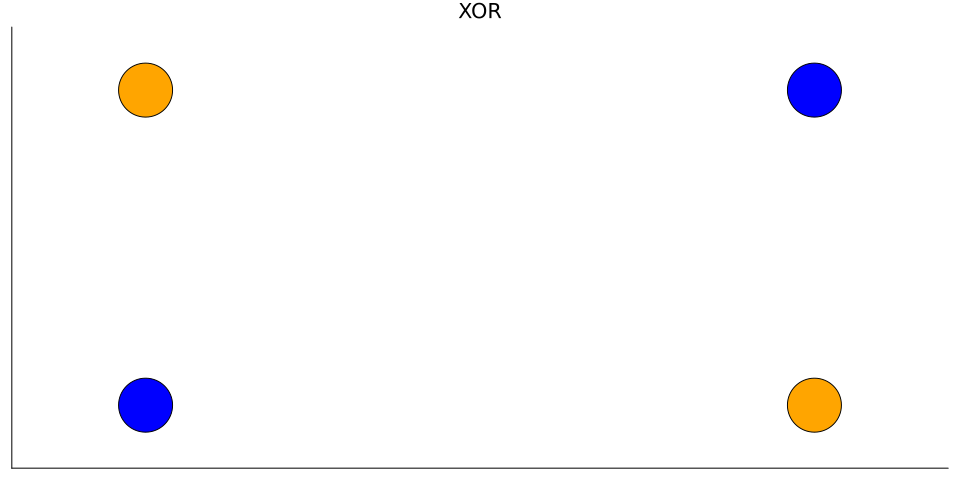
\includegraphics{lecture2_files/figure-beamer/cell-15-output-1.pdf}

\begin{itemize}
\tightlist
\item
  The false values are indicated in blue and the true values in orange.
\item
  There is \emph{no} line that can be drawn to seperate blues and
  oranges.
\end{itemize}
\end{frame}

\begin{frame}{Two layers: solving XOR}
\protect\hypertarget{two-layers-solving-xor}{}
\begin{itemize}
\item
  To solve the XOR problem we need to augment the perceptron.
\item
  We do this by having two layers of perceptrons and feed the output of
  one into the other.
\item
  We \emph{need} the activation function to be non-linear (otherwise it
  will reduce to a single perceptron layer).
\item
  This is no longer performs linear regression.
\end{itemize}

\note{Give the students a few minutes to try and solve this with two
layers and the hint of using a ReLu.}
\end{frame}

\begin{frame}[fragile]{The solution:}
\protect\hypertarget{the-solution}{}
\begin{Shaded}
\begin{Highlighting}[]
\FunctionTok{relu}\NormalTok{(x) }\OperatorTok{=}\NormalTok{ x }\OperatorTok{.*}\NormalTok{ (x }\OperatorTok{.\textgreater{}} \FloatTok{0}\NormalTok{)}
\FunctionTok{layer1}\NormalTok{(x) }\OperatorTok{=} \FunctionTok{relu}\NormalTok{([}\FloatTok{1} \OperatorTok{{-}}\FloatTok{1}\NormalTok{; }\OperatorTok{{-}}\FloatTok{1} \FloatTok{1}\NormalTok{] }\OperatorTok{*}\NormalTok{ x)}
\FunctionTok{layer2}\NormalTok{(x) }\OperatorTok{=}\NormalTok{ [}\FloatTok{1} \FloatTok{1}\NormalTok{] }\OperatorTok{*}\NormalTok{ x}
\FunctionTok{xor}\NormalTok{(x) }\OperatorTok{=} \FunctionTok{layer2}\NormalTok{(}\FunctionTok{layer1}\NormalTok{(x))}
\FunctionTok{xor}\NormalTok{.([[}\FloatTok{0}\NormalTok{,}\FloatTok{0}\NormalTok{], [}\FloatTok{0}\NormalTok{,}\FloatTok{1}\NormalTok{], [}\FloatTok{1}\NormalTok{,}\FloatTok{0}\NormalTok{], [}\FloatTok{1}\NormalTok{,}\FloatTok{1}\NormalTok{]])}
\end{Highlighting}
\end{Shaded}

\begin{verbatim}
4-element Vector{Vector{Int64}}:
 [0]
 [1]
 [1]
 [0]
\end{verbatim}
\end{frame}

\begin{frame}{Multi-Layer Perceptrons: General Artificial Neural
Networks.}
\protect\hypertarget{multi-layer-perceptrons-general-artificial-neural-networks.}{}
\begin{itemize}
\item
  When multiple layers of perceptrons are chained together they are
  called: \emph{multi-layer perceptrons} (MLPs).
\item
  These are the most general form of \emph{artificial neural networks}
  (ANNs).
\end{itemize}
\end{frame}

\begin{frame}{}
\protect\hypertarget{section-5}{}
\begin{itemize}
\item
  They can be used to model \emph{any} function and are thus universal
  models.
\item
  When they have many layers they are considered ``deep'' thus the name
  Deep Learning.
\item
  We need a way to teach them.
\end{itemize}
\end{frame}

\begin{frame}{Summary.}
\protect\hypertarget{summary.}{}
\begin{itemize}
\item
  Biological models of neurons exist from highly realistic and
  expensive, to cheap but less accurate.
\item
  Neurons can be modelled as a network and this can perform any function
  (with training).
\item
  The Hopfield network is a simple setup with a biological training rule
  that explains much of brain function.
\item
  The perceptron is an easy to train biologically inspired linear
  regression model.
\item
  The multi-layer perceptron is an all-purpose statistical model.
\end{itemize}
\end{frame}



\end{document}
